\section{Results}

An initial goal of this project was to create a model of my head for 3d printing,
but it was difficult to keep a consistent posture for multiple angles.
\begin{figure}[h]
\centering
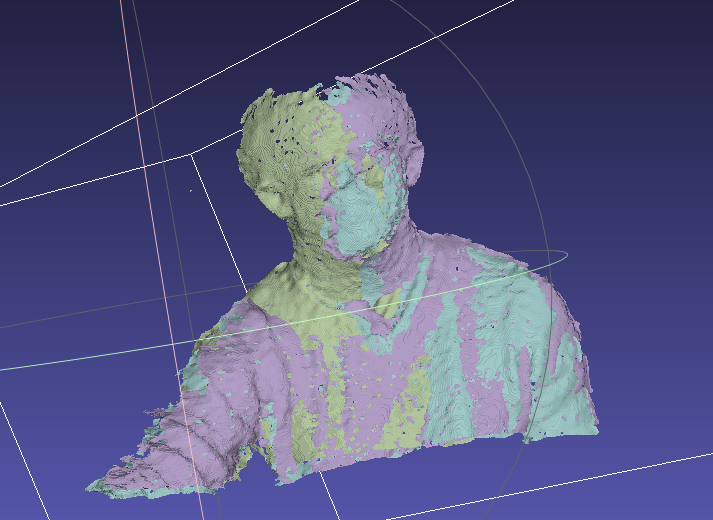
\includegraphics[width=0.6\textwidth]{poor_alignment.png}
\caption{Difficult to take depth selfies from different angles without moving}
\end{figure}
Photography skill (and a longer USB cable!) would be helpful for capturing quality depth images.
When the object is not rigid across different frames the point clouds do not quite fit together.

For the Cube Man project, the final reconstructions are somewhat disappointing.
None of the reconstruction methods tried reconstruct a smooth but detailed model.
Even after carefully aligning multiple clouds the reconstruction obtained
from the merged point clouds is jagged and full of artifacts.

The reality is that these devices do not have very good accuracy at small scales.
The infrared emitter mitigates some of the problems of stereoscopic depth but
also seem to introduce some noise.

However, the D435 and like can produce a stream of decent depth images
at high speed.  Obviously, the Fusion method \cite{newcombe2011kinectfusion}
is superior to this artisanal approach. With a big data streaming approach,
it is possible to identify noise, discard erroneous values and fill in holes and details.
